\documentclass[]{scrartcl}
\usepackage[utf8]{inputenc}
\usepackage{graphicx}
\usepackage{amsmath}
\usepackage{float}

\title{Technik und Technologie vernetzter Systeme  \\ Abgabe der Praktikumsaufgabe 1}

\author{Maria Lüdemann und Birger Kamp}

\begin{document}

\maketitle

\section{Projektschritt 1}
Nach der Durchführung des Projektschritts 1 anhand des Szenarios 1 haben wir einen Wireshark Mitschnitt gespeichert der die Unterhaltung der Bestandteile des Netzwerks mitschneidet. Der Mitschnitt ist unten aufgeführt.

\begin{figure}[H]
	\centering
	\includegraphics[width=1\linewidth]{wireshark_1.png}
	\label{fig:wireshark_1}
\end{figure}

Hier zu sehen ist der Ablauf des Neighbor Solicitation Protokolls. Der Abblauf wird im folgenden Flussdiagramm noch einmal verdeutlicht. 


\begin{figure}[H]
	\centering
	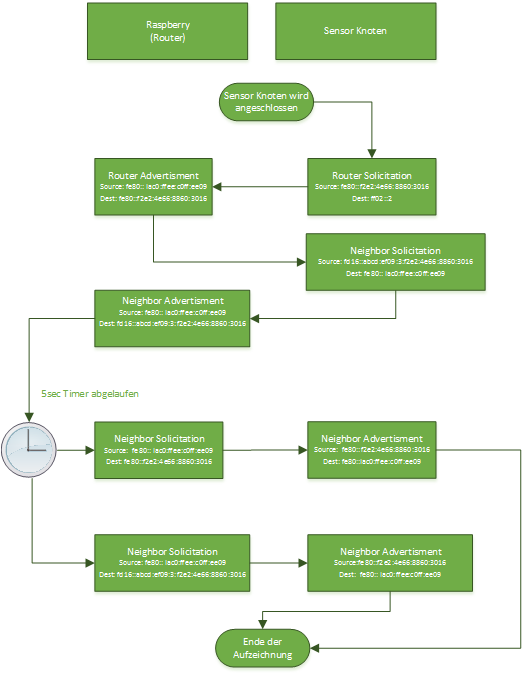
\includegraphics[width=1\linewidth]{flussdiagramm.png}
	\label{fig:flussdiagramm}
\end{figure}

Hier zu sehen ist

\textbf{Auffälligkeit}\\
Nach RFC 6775 (Abschnitt 3.3) sendet der Host einen NS an den Router mit einer gewissen Lifetime. Sollte die Lifetime ablaufen, dann erneuert der Host diesen Eintrag. Der Router fragt nicht aktiv nach beim Host. Die Schritte 3 und 4 sollten nach RFC 6775 nicht passieren!


\section{Projektschritt 2}

\section{Projektschritt 3}

\end{document}